\documentclass[11pt]{article}

\usepackage[margin=1in]{geometry}
\usepackage[T1]{fontenc}
\usepackage{lmodern}
\usepackage{amsmath,amssymb,amsthm}
\usepackage{booktabs}
\usepackage{array}
\usepackage{multirow}
\usepackage{graphicx}
\graphicspath{{figures/}{report/figures/}}
\usepackage{xcolor}
\usepackage{enumitem}
\usepackage[colorlinks=true,linkcolor=blue!50!black,citecolor=magenta,urlcolor=blue!50!black]{hyperref}
\usepackage[labelfont=bf]{caption}
\renewcommand{\figurename}{Fig.}

\newcommand{\R}{\mathbb{R}}
\newcommand{\dB}{\,\mathrm{dB}}

\title{What Determines the Effectiveness of 3D Field of Junctions?}
\author{Samudraneel Sarkar, Sakshi Patil$^{*}$, Nikhil Kumar$^{*}$,
Manpreet Singh$^{*}$\\[1.4em]
MNNIT Allahabad\\
{\small\texttt{\{samudraneel.20233249, patil.20233209, nikhil.20233202,
manpreet.20233180\}@mnnit.ac.in}}}
\date{}

\begin{document}
\maketitle
\begingroup\renewcommand{\thefootnote}{}%
\footnotetext{$^{*}$Equal contribution; order determined by coin flip.}%
\endgroup

\begin{abstract}
We study when the 3D Field of Junctions (FoJ) denoiser helps and when it
fails. FoJ fits each patch of a volume with a junction of planar wedges
and averages the overlapping fits; it requires no training data and is
designed for low-SNR volumes. We find that the released implementation,
at its default configuration, reduces to an independent fit per patch
followed by averaging, with no inter-patch coupling. From this mechanism
follow three requirements for FoJ to help, each verified experimentally
on CT reconstruction and three new denoising domains.
First, the input must be unbiased: each region intensity is a mean of
the voxels it covers, so a systematic offset in the input is reproduced
rather than removed. Second, the structure must be piecewise-flat at or
above the patch scale; features smaller than the patch cannot be
represented by wedges, and the output collapses toward the mean. Third,
the input noise must be high enough that the wedge model's bias is paid
for by the noise it removes.
\end{abstract}

%=====================================================================
\section{Introduction}

Volumetric imaging modalities operate under dose and acquisition-time
limits that keep the signal-to-noise ratio (SNR) low: CT scans limit the
X-ray dose to reduce radiation exposure~\cite{lepcha2025low}, lower-cost
MRI systems use weaker magnetic fields~\cite{arnold2023low}, and electron
tomography limits electron counts to avoid sample
damage~\cite{turk2020promise}. Denoising is therefore a routine step in
volume analysis. The classical toolbox includes local filters such as
Gaussian smoothing
and median filtering; variational methods such as total-variation (TV)
minimization~\cite{rudin1992nonlinear,chambolle2004algorithm}, which
favor piecewise-constant solutions; and patch-recurrence methods such as
non-local means~\cite{buades2005nonlocal} and
BM3D~\cite{dabov2007image}. Learned denoisers trained on paired
data~\cite{zhang2017beyond} currently dominate at moderate noise levels.

Field of Junctions (FoJ)~\cite{verbin2021foj} is a training-free structural
prior for image denoising. It models each small image patch as a few
constant-intensity regions separated by straight boundaries that meet at a
vertex, called a junction, and produces a denoised image by averaging the
overlapping patch models. 3D FoJ~\cite{moeini2026foj3d} extends the model
to volumes: three planes meeting at a common vertex divide each cubic patch
into constant-valued wedges. Because the wedge model captures sharp
surfaces and corners rather than smooth content, it is designed for the
low-SNR regime; the authors demonstrate it on low-dose X-ray CT,
cryo-electron tomography, and point-cloud denoising
(Figure~\ref{fig:teaser}), and report that it outperforms the baselines
evaluated in their study: classical regularization, untrained neural
representations~\cite{ulyanov2018deep,zha2022naf}, and a denoiser trained
on noisy data alone~\cite{noise2noise,filter2noise}. A learned 2D
successor, Boundary Attention~\cite{polansky2024boundary},
chooses patch sizes adaptively.

\begin{figure}[t]
\centering
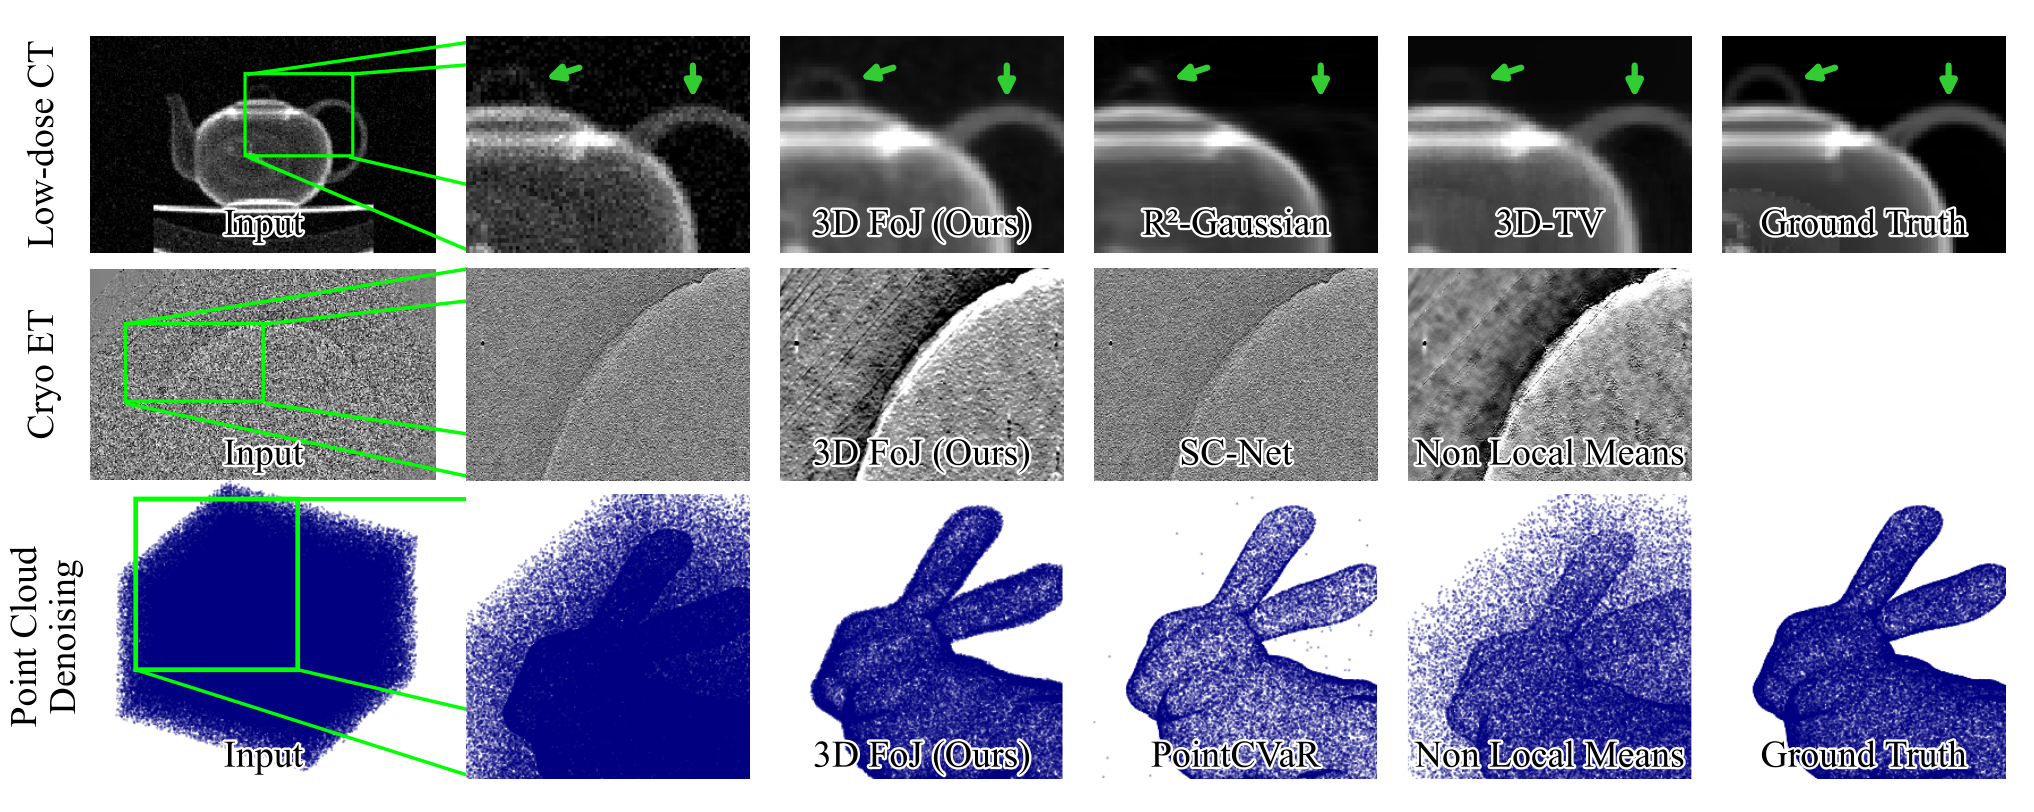
\includegraphics[width=\linewidth]{ext/cvpr_teaser.png}
\caption{Applications of 3D FoJ demonstrated in the original paper:
low-dose CT (top), cryo-ET (middle), and point-cloud denoising (bottom).
Figure reproduced from~\cite{moeini2026foj3d} (CC~BY~4.0).}
\label{fig:teaser}
\end{figure}

These demonstrations show that FoJ \emph{can} work well on low-SNR
volumes, but they do not characterize the conditions under which it does.
The method's main hyperparameter is the patch size $R$; the reported
ablation finds reconstruction quality increasing monotonically with $R$
on a low-dose CT task, and conjectures that the optimal patch size grows
with noise level. Whether that holds, and more generally what determines
when the method helps at all, is the subject of this report.

Our approach is to first establish what the algorithm actually computes
at the configuration used for the published results
(Section~\ref{sec:mechanism}), and then to test the conditions that
follow from it. Reproducing the CT ablation required re-implementing the
simulation pipeline, since the public
repository\footnote{\url{https://github.com/voilalab/3D-Field-of-Junctions}}
releases the
FoJ model but not the CT simulation, CGLS settings, view angles, or the
$M{=}3$ region model used in the paper. We rebuild it following the
R$^2$-Gaussian benchmark~\cite{zha2024r2gaussian} whose data generator
the paper used, and evaluate the released FoJ code on that task plus
three denoising domains the paper did not test: BrainWeb MRI, grayscale
micro-CT of Bentheim sandstone, and two binary porous-media volumes.
Our implementation and experiment scripts are available in the
accompanying repository.\footnote{\url{https://github.com/samudraneel05/foj3d-factor-study}}

%=====================================================================
\section{The 3D FoJ model}
\label{sec:model}

Let $y\in\R^{N^3}$ be a noisy volume and let $\{\Omega_p\}_{p}$ be cubic
patches of side $R$ on a grid with stride $s$. Each patch $p$ carries
parameters $\theta_p$ (three plane orientations and a shared vertex, nine
numbers), which define soft indicator functions $u_{p,k}(\cdot;\theta_p)$
of $M$ regions. Given $\theta_p$, the region intensities are
indicator-weighted means,
\begin{equation}
  c_{p,k} = \frac{\sum_{x\in\Omega_p} u_{p,k}(x)\,y(x)}{\sum_{x\in\Omega_p} u_{p,k}(x)},
  \label{eq:colors}
\end{equation}
and the patch rendering is $\hat y_p(x)=\sum_k u_{p,k}(x)c_{p,k}$. The full
objective is
\begingroup\postdisplaypenalty=10000
\begin{equation}
  \mathcal{L}(\theta)=\sum_p \Big[\underbrace{\|\hat y_p - y|_{\Omega_p}\|_2^2}_{\text{data}}
  + \lambda_B\,\mathcal{C}^{B}_p(\theta) + \lambda_C\,\mathcal{C}^{C}_p(\theta)\Big],
  \label{eq:loss}
\end{equation}
where $\mathcal{C}^B,\mathcal{C}^C$ penalize disagreement between a patch's
boundary and colour maps and the current global estimates.\endgroup{} The
output is the uniform average of overlapping renderings,
\begin{equation}
  \hat x(x)=\frac{1}{|\{p: x\in\Omega_p\}|}\sum_{p:\,x\in\Omega_p}\hat y_p(x).
  \label{eq:avg}
\end{equation}
Optimization has two phases: $N_{\text{init}}$ \emph{initialization}
iterations (coordinate descent over the nine parameters on a discrete grid,
then a vertex line search along each plane normal) and $N_{\text{ref}}$
\emph{refinement} iterations (Adam on Eq.~\eqref{eq:loss}). The default
used for the paper's results is $N_{\text{init}}{=}N_{\text{ref}}{=}1$,
$R{=}10$, $s{=}2$, $M{=}3$; the released code implements $M{=}2$, one
convex wedge and its complement.

\begin{figure}[t]
\centering
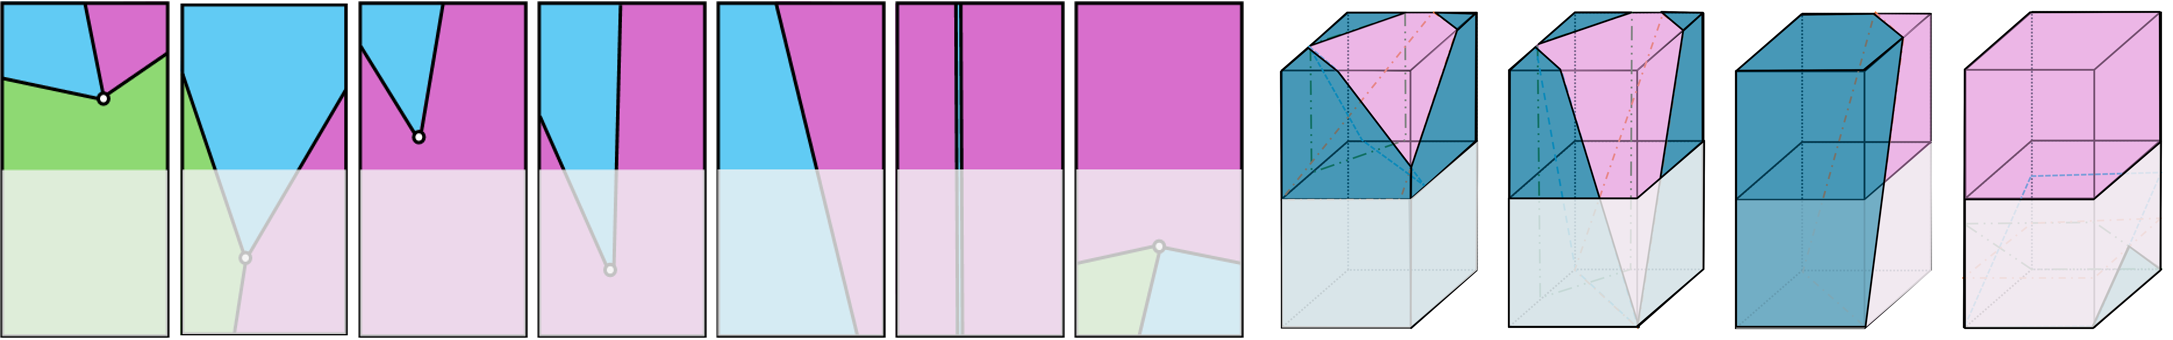
\includegraphics[width=\linewidth]{ext/fig_junction_full.png}
\caption{Junction schematics, reproduced from~\cite{moeini2026foj3d}
(CC~BY~4.0). Left: 2D FoJ with $M{=}3$ regions; a vertex placed inside,
on the boundary of, or outside the patch produces a three-way junction, a
single edge, or a constant region, so the same model expresses all three
local geometries. Right: the 3D FoJ variant, in which three planes
meeting at a vertex divide the cubic patch into constant-valued wedges
($M{=}2$ shown).}
\label{fig:junction}
\end{figure}

%=====================================================================
\section{The effective estimator}
\label{sec:mechanism}

Before examining when FoJ helps, we first establish what the algorithm
computes at the configuration used for the published results, since the
conditions under which the method can succeed follow from the estimator
itself.

Equation~\eqref{eq:loss} describes a coupled system: the boundary- and
color-consistency terms tie each patch to the global estimates, so
neighboring junctions are meant to agree on where surfaces lie and what
intensities they take. That coupling is what makes the method a
\emph{field} of junctions rather than a collection of independent ones.
At the configuration released by the authors and used for the published
results, however, this coupling never engages, for two reasons. The
consistency weights are ramped in only when the refinement stage runs
for more than one iteration; the released schedule uses exactly one, so
$\lambda_B$ and $\lambda_C$ remain zero throughout and the consistency
terms contribute nothing. And the single refinement step that does run
re-renders the volume from parameter values computed before the
optimizer's update, so even it leaves the output unchanged.

What runs in practice is therefore simpler than the objective suggests:
each patch is fitted independently,
\begin{equation}
  \theta_p^\star = \operatorname*{arg\,min}_{\theta}\
  \|\hat y_p(\theta) - y|_{\Omega_p}\|_2^2,
  \label{eq:perpatch}
\end{equation}
and the denoised volume is the average of the overlapping fits
(Eq.~\eqref{eq:avg}).

This description is directly checkable. If patches never interact, the
output cannot depend on how they are grouped: processing the volume in
spatial chunks, each padded so that every patch sees its full support,
reproduces the global implementation to $\sim\!3\times10^{-7}$ on a CGLS
reconstruction crop, and switching the refinement step on or off changes
the output by at most $3.6\times10^{-7}$. The paper's own ablations are
consistent with the same picture: batch sizes 1--6 give identical
results, and additional refinement iterations, which are what activate
the consistency terms, degrade rather than improve quality. All
full-volume results reported below are within $0.01\dB$ of an exact
global run.

The consequences for effectiveness are immediate. An estimator that only
replaces each wedge of the input with a regional mean has no way to
remove a \emph{bias} already present in that input: the mean reproduces
the offset rather than correcting it. It can only represent structure
that is \emph{piecewise-flat at the patch scale}: smooth texture and
features smaller than $R$ are averaged away. And its benefit is bounded
by its bias: the wedge model is a coarse approximation, so it helps only
where the noise it removes exceeds the error it introduces. The
experiments of Section~\ref{sec:experiments} test each of these
conditions in turn.

%=====================================================================
\section{Experimental setup}
\label{sec:setup}

\paragraph{CT reconstruction.}
We reconstruct the $256^3$ \emph{engine} volume from 20 cone-beam views
corrupted by Poisson noise, then apply FoJ, following the ablation of
Table~3 in~\cite{moeini2026foj3d} (reproduced here as
Table~\ref{tab:paper}). The view angles, CGLS settings, and any
preprocessing of the reconstruction are not specified in the paper, so we
fix: the R$^2$-Gaussian scanner geometry (cone beam, source--detector
distance 7, source--object distance 5, $256\times256$ detector); twenty
stratified-jitter angles in $[0,2\pi)$, seed 0; Poisson noise as in
TIGRE's~\cite{biguri2016tigre} \texttt{CTnoise} with $P{=}50$ expected
photons per pixel in air
(``P50''), defined relative to the maximum projection value; and
CGLS~\cite{hestenes1952cg} with 60 iterations. FoJ runs at $M{=}2$,
$N_{\text{init}}{=}N_{\text{ref}}{=}1$, stride 2,
$R\in\{4,6,8,10,12\}$, executed in halo-padded chunks on a single A100;
one $256^3$ run takes 225--325\,s. Metrics are full-volume 3D PSNR (peak
1) and MS-SSIM~\cite{wang2003msssim} averaged over 360 forward
projections.

\begin{table}[t]
\centering
\caption{Reported results for the ablation we reproduce (engine, P50,
$M{=}3$, batch 6, stride 2; Table~3 of~\cite{moeini2026foj3d}).}
\label{tab:paper}
\begin{tabular}{lccccc}
\toprule
$R$ & 4 & 6 & 8 & 10 & 12 \\
\midrule
PSNR (dB) & 11.33 & 14.37 & 16.18 & 17.17 & 17.70 \\
MS-SSIM   & 0.762 & 0.784 & 0.796 & 0.798 & 0.800 \\
Runtime (min, RTX A6000) & 7.2 & 10.5 & 13.1 & 17.2 & 24.7 \\
\bottomrule
\end{tabular}
\end{table}

\paragraph{Volume denoising.}
We run direct denoising on three domains with public ground truth: a
$192^3$ crop of Bentheim sandstone micro-CT ($5.85\,\mu\mathrm{m}$
voxels, grains tens of voxels across~\cite{bentheim2015zenodo}) under
additive Gaussian noise at $\sigma\in\{15\%,30\%,40\%,55\%\}$ of the
dynamic range; the BrainWeb T1 phantom
($181{\times}217{\times}181$~\cite{collins1998brainweb}) under Rician
noise at $\sigma\in\{3\%\ldots13\%\}$; and two binary porous-media
volumes (a synthetic sphere pack and a segmented Berea
scan~\cite{neumann2020sandstones}) with feature sizes of about 2~voxels,
under Gaussian noise at $\sigma{=}15\%$. Baselines are Gaussian
filtering, a $3^3$ median filter, and
TV~\cite{rudin1992nonlinear,chambolle2004algorithm} at three weights, all under
identical conditions; FoJ runs at $R\in\{6,8,12\}$, stride 2. We also
report a boundary F-score over gradient-magnitude edge voxels, since edge
preservation is FoJ's distinguishing feature.

%=====================================================================
\section{Experiments}
\label{sec:experiments}

\subsection{Input bias: clamping the reconstruction}
\label{sec:bias}

By Eq.~\eqref{eq:colors}, every region intensity is a mean of the input
voxels it covers, so a systematic offset in the input passes straight
through the model. The natural source of bias in the CT pipeline is
clamping: CGLS noise in the near-zero background is roughly symmetric,
and clipping the reconstruction to $[0,1]$ deletes the negative half,
leaving a positive offset.

Table~\ref{tab:tigre} shows the effect. Clamping raises the \emph{input}
PSNR by $3\dB$ but lowers the FoJ output by $2.7\dB$ ($R{=}6$) to
$4.3\dB$ ($R{=}12$), and almost flattens the patch-size trend
($0.37\dB$ between $R{=}6$ and $R{=}12$). Larger patches average more
background voxels into each region estimate, so they lose the most from
the biased input. The reported values lie between our clamped and
unclamped rows, so the authors' preprocessing choice cannot be inferred.

\begin{table}[t]
\centering
\caption{Engine $256^3$, 20 jittered views, P50, TIGRE CGLS-60, released
FoJ ($M{=}2$), stride 2. CGLS input PSNR: $6.92\dB$ unclamped, $9.97\dB$
clamped; input MS-SSIM 0.682. ``--'': run lost to a VM preemption.}
\label{tab:tigre}
\begin{tabular}{lccccc}
\toprule
$R$ & 4 & 6 & 8 & 10 & 12 \\
\midrule
Reported ($M{=}3$), PSNR            & 11.33 & 14.37 & 16.18 & 17.17 & 17.70 \\
\midrule
Ours, unclamped input, PSNR         & 14.72 & 16.93 & 17.99 & 18.58 & \textbf{18.86} \\
Ours, unclamped input, MS-SSIM      & 0.786 & 0.829 & 0.854 & 0.870 & \textbf{0.880} \\
\midrule
Ours, clamped input, PSNR           & --    & 14.24 & 14.48 & 14.58 & \textbf{14.61} \\
Ours, clamped input, MS-SSIM        & --    & 0.723 & 0.728 & \textbf{0.728} & 0.726 \\
\midrule
Gap ours (unclamped) $-$ reported, PSNR & $+3.39$ & $+2.56$ & $+1.81$ & $+1.41$ & $+1.16$ \\
\bottomrule
\end{tabular}
\end{table}

With an unclamped input, the qualitative trend reproduces: PSNR and
MS-SSIM increase monotonically with $R$, $R{=}12$ is best, and the
marginal gains shrink ($+2.2$, $+1.1$, $+0.6$, $+0.3\dB$ versus the
reported $+3.0$, $+1.8$, $+1.0$, $+0.5\dB$). Our absolute values are
$1.2$--$3.4\dB$ higher; the region count ($M{=}2$ versus $M{=}3$)
accounts for at most about $0.14\dB$ by the reported region ablation.

\subsection{Structure compatibility}
\label{sec:structure}

The wedge model expresses flat regions with hard boundaries at roughly
the patch scale or larger. Three tests probe this requirement, one on the
input's artifact structure and two on the volume's own structure.

\paragraph{Artifact structure: the patch-size ordering reverses.}
Re-running the ablation with a simplified pure-PyTorch cone-beam
projector (trilinear sampling along rays) in place of TIGRE changes the
ordering. The simplified projector scales line integrals by $2.41\times$
and rotates about a different volume axis, so the noise model, defined
relative to the maximum projection value, produces artifacts of
different shape and level at matched nominal noise. With CGLS-15 and
P50, its input reaches $12.20\dB$ clamped ($9.38\dB$ unclamped),
comparable to the TIGRE input, yet $R{=}6$ or $R{=}8$ is now best and
$R{=}12$ is worst (Table~\ref{tab:inhouse}). A CGLS-iteration sweep
never recovers a monotone trend. Two inputs of similar PSNR thus yield
opposite hyperparameter conclusions: FoJ responds to the structure of
the artifacts, not their energy. Consistent with this, a crop sweep on
the R$^2$-Gaussian \emph{foot} and \emph{jaw} volumes with the same
projector puts the best $R$ at 6--8 for engine and foot but 10--12 for
jaw at every noise level; in these runs object scale, not noise level,
sets the optimal patch size.

\begin{table}[t]
\centering
\caption{The same FoJ settings on CGLS-15 inputs from the simplified
projector (engine $256^3$, P50). The ordering is the opposite of
Table~\ref{tab:tigre}.}
\label{tab:inhouse}
\begin{tabular}{lccccc}
\toprule
$R$ & 4 & 6 & 8 & 10 & 12 \\
\midrule
Clamped input, PSNR   & 17.53 & \textbf{17.84} & 17.77 & 17.64 & 17.48 \\
Unclamped input, PSNR & 20.70 & 22.22 & \textbf{22.28} & 22.11 & 21.74 \\
\bottomrule
\end{tabular}
\end{table}

\paragraph{Smooth texture: MRI fails at every noise level.}
On BrainWeb T1 under Rician noise, FoJ never reaches the classical
baselines. At $\sigma{=}3\%$ it trails a $3^3$ median filter by $5.1\dB$;
at $\sigma{=}13\%$ the gap shrinks to $1.0\dB$ but never closes, and the
ordering is $R{=}6>8>12$: larger patches quantize away more of the
tissue texture that the wedge model cannot represent. The same holds
when FoJ serves as the denoiser in a plug-and-play loop for accelerated
MRI; at $4\times$ undersampling it reaches $28.0\dB$ against $30.4\dB$
for TV-PnP.

\paragraph{Sub-patch-scale structure: total collapse.}
On the two binary volumes, features are about 2~voxels across, far below
any tested patch size. FoJ collapses toward the global mean: output
standard deviation $0.09$ against $0.49$ for the input, and $7.1\dB$
against the noisy input's own $19.5\dB$. When an $R$-voxel patch
contains only unmodelable speckle, its best fit is a constant
(Figure~\ref{fig:collapse}), and averaging constants returns a constant.

\begin{figure}[t]
\centering
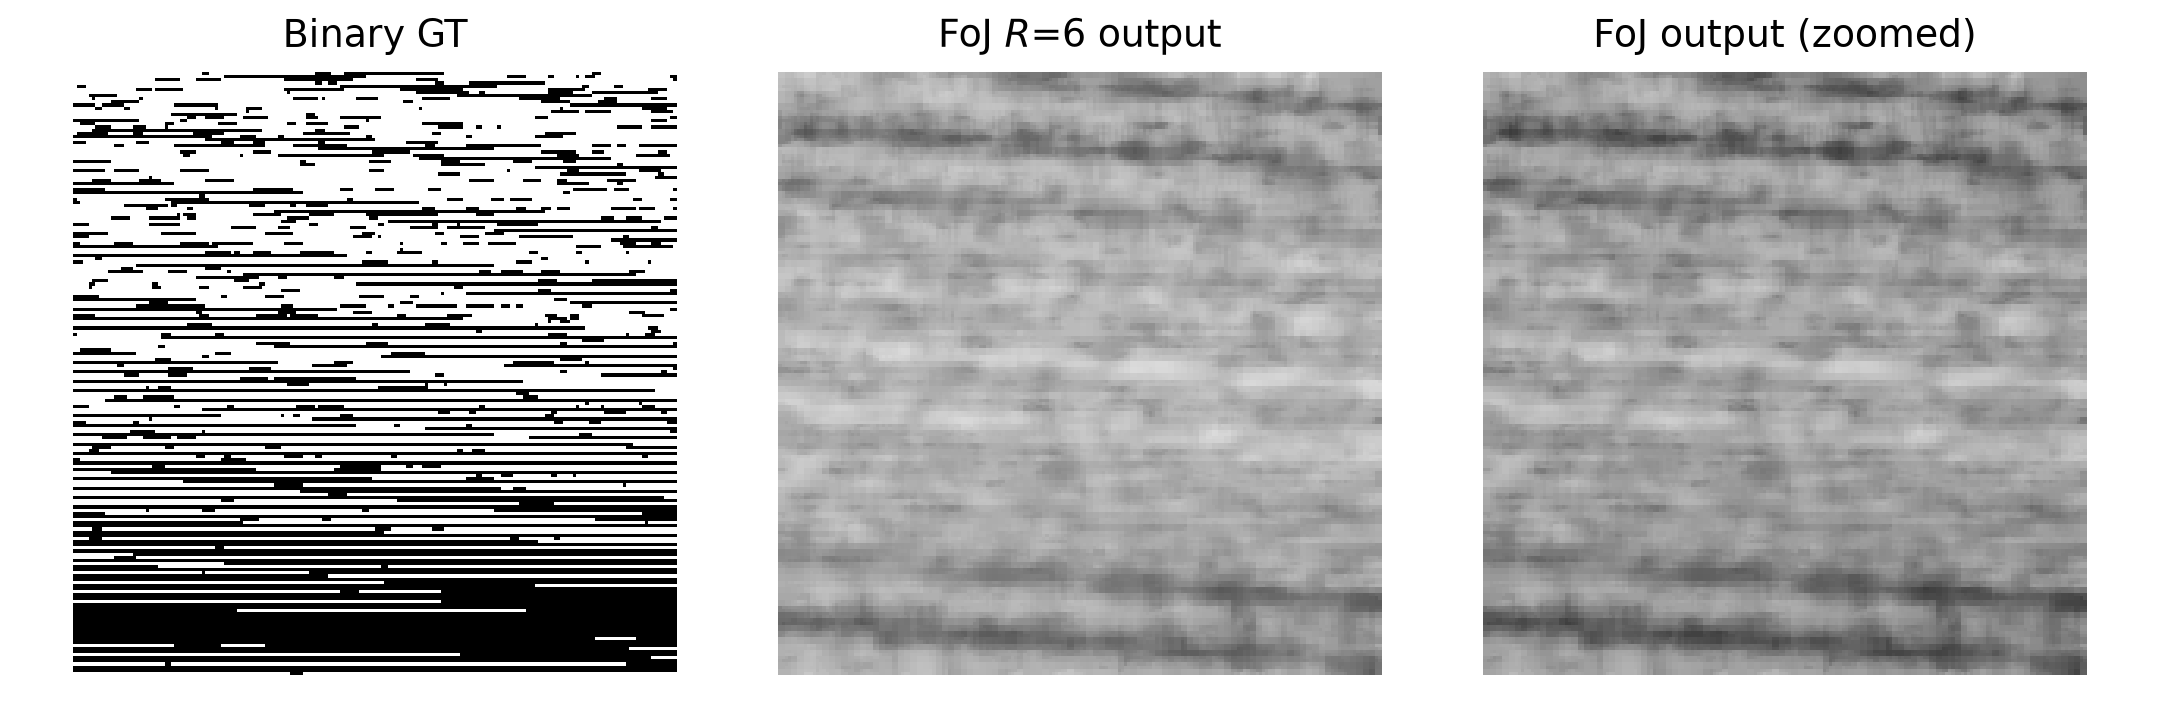
\includegraphics[width=\linewidth]{fig_collapse.png}
\caption{Collapse on sub-patch-scale binary structure. Left: GT
mid-slice (features about 2 voxels). Centre/right: FoJ $R{=}6$ output;
only the coarsest layer structure survives and fine texture is averaged
away.}
\label{fig:collapse}
\end{figure}

\subsection{Noise regime: the crossover}
\label{sec:snr}

If FoJ carries a large approximation bias, it should lose whenever
classical filters can recover the signal from local statistics alone,
and win only where those filters break down. Bentheim micro-CT provides
the compatible-structure test case: grains and pores are near-constant
regions tens of voxels across.

\begin{table}[t]
\centering\small
\begin{tabular}{lrrrrr}
\toprule
$\sigma$ & Noisy & Gaussian & Median & TV (best $w$) & FoJ (best $R$)\\
\midrule
15\% & 16.89 & \textbf{28.51} & 27.01 & 27.65 & 26.55\\
30\% & 12.00 & 25.26 & 22.26 & \textbf{26.03} & 25.64\\
40\% & 10.28 & 23.39 & 20.04 & 23.32 & \textbf{24.93}\\
55\% & \phantom{0}8.76 & 21.05 & 17.60 & 16.30 & \textbf{24.29}\\
\bottomrule
\end{tabular}
\caption{PSNR (dB) on the Bentheim volume. FoJ overtakes all classical
baselines once the input PSNR falls below ${\sim}11$~dB ($+1.5$~dB at
$\sigma{=}40\%$, $+3.2$~dB at $\sigma{=}55\%$) while trailing at moderate
noise.}
\label{tab:bentheim}
\end{table}

Table~\ref{tab:bentheim} and Figure~\ref{fig:curve} show a clean
crossover. FoJ trails at $\sigma\le30\%$, overtakes every classical
baseline between 30\% and 40\%, and its margin grows with noise. The
advantage is concentrated at boundaries: at $\sigma{=}55\%$ FoJ retains
boundary-F1 $=0.85$--$0.88$ against $0.54$ for the best TV weight, and
Figure~\ref{fig:slices} shows the grain--pore interfaces preserved where
TV loses them. The ordering at $\sigma{=}55\%$ is $R{=}8>6>12$.

The same concentration appears inside the published results. The
per-dataset table in~\cite{moeini2026foj3d} shows FoJ with the best PSNR
on three of the five CT volumes at its lowest noise level (P50), on none
of them at the next level (P100), and losing at every level on two
volumes; the accompanying text likewise describes the higher-SNR results
as mixed. The measured advantage of FoJ in the published data is thus
confined to the same regime our experiments identify.

\begin{figure}[t]
\centering
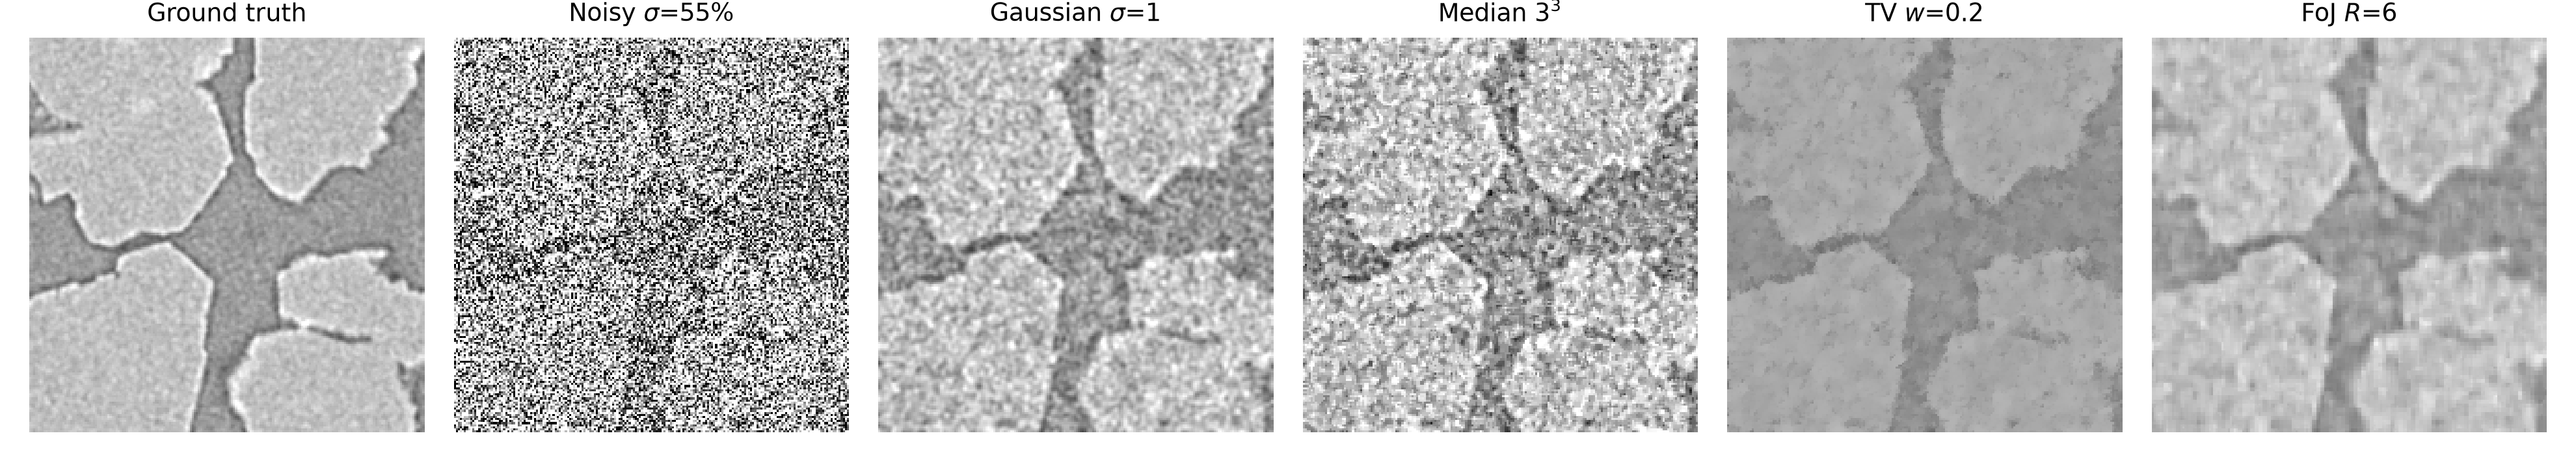
\includegraphics[width=\linewidth]{fig_slices.png}
\caption{Bentheim micro-CT, mid-slice, $\sigma{=}55\%$ Gaussian noise.
FoJ ($R{=}6$) preserves the sharp grain--pore interfaces that Gaussian,
median, and TV filtering blur.}
\label{fig:slices}
\end{figure}

\begin{figure}[t]
\centering
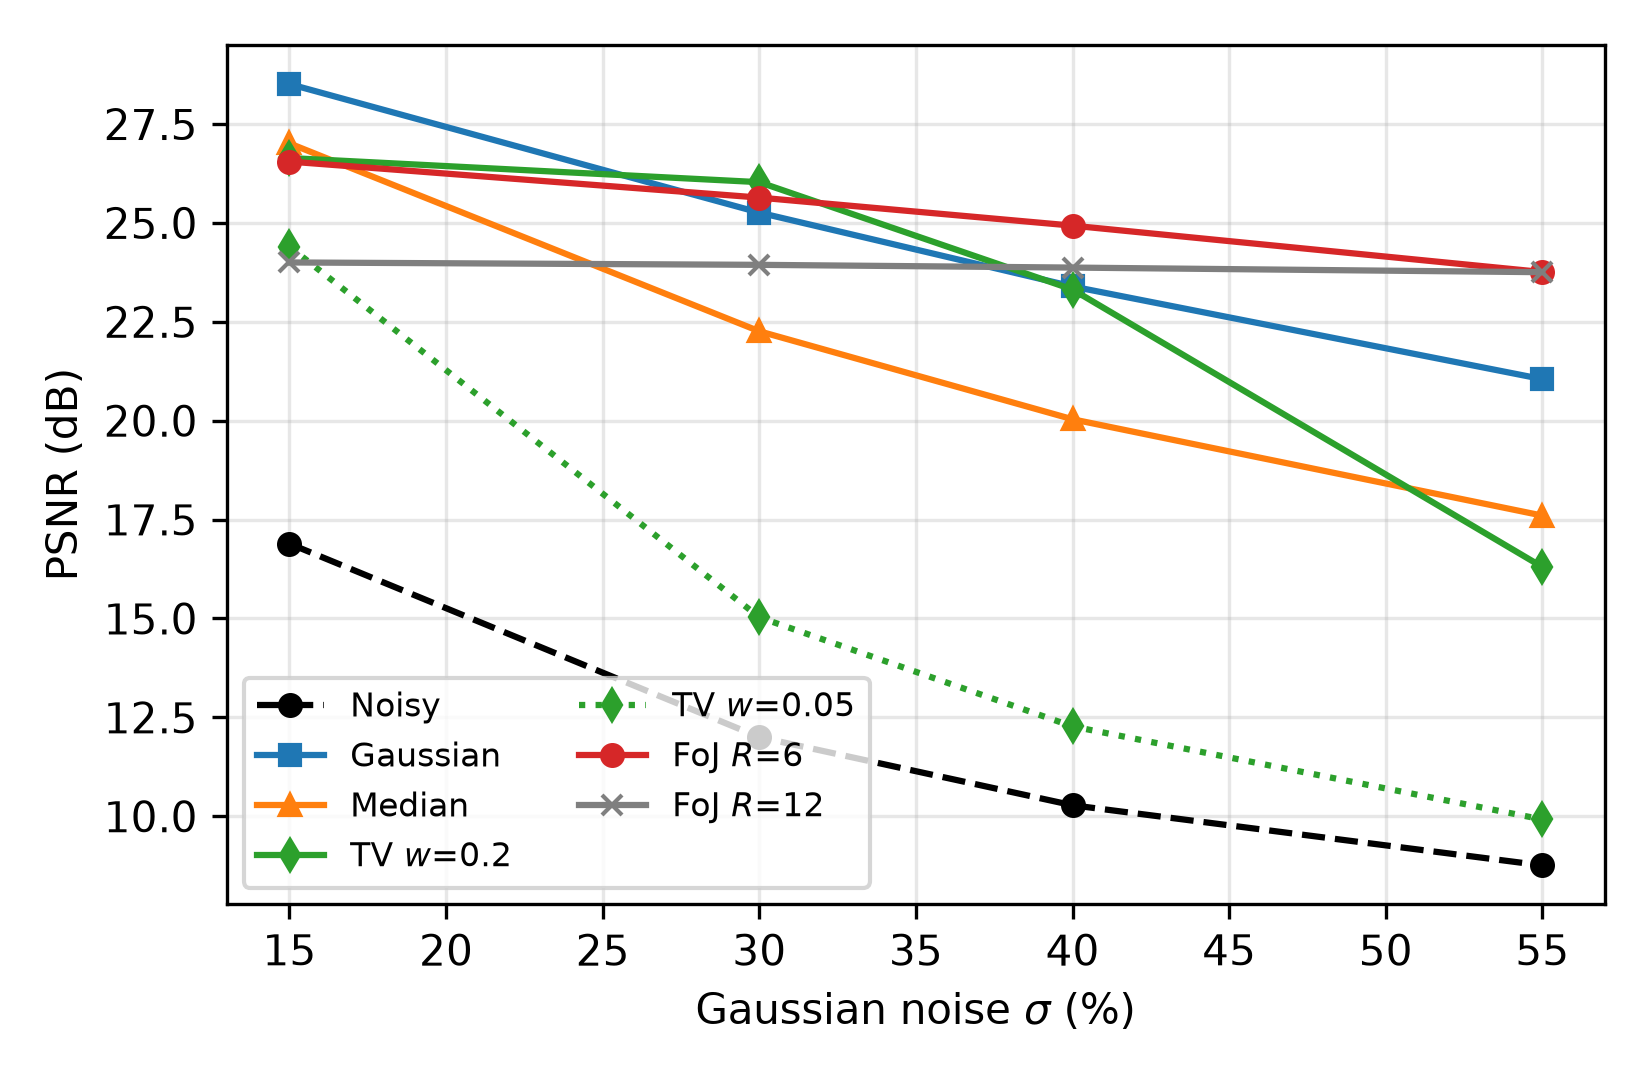
\includegraphics[width=0.72\linewidth]{fig_curve.png}
\caption{PSNR versus noise level on Bentheim micro-CT. FoJ (red)
overtakes the classical filters between $\sigma{=}30\%$ and $40\%$.}
\label{fig:curve}
\end{figure}

Figure~\ref{fig:domains} places all the denoising results on one axis:
FoJ's margin over the best classical filter versus input PSNR. On
compatible structure the margin grows monotonically with noise and
crosses zero at an input PSNR of ${\approx}11\dB$, which is also the
operating regime of the reported CT experiments: their inputs are
${\sim}10\dB$ CGLS volumes. MRI stays negative throughout, because its
violation is structural rather than noise-driven. On volumetric data
with phase-scale structure and input PSNR $\lesssim 11\dB$, the released
3D FoJ implementation outperforms Gaussian, median, and TV denoising by
up to $3.2\dB$.

\begin{figure}[t]
\centering
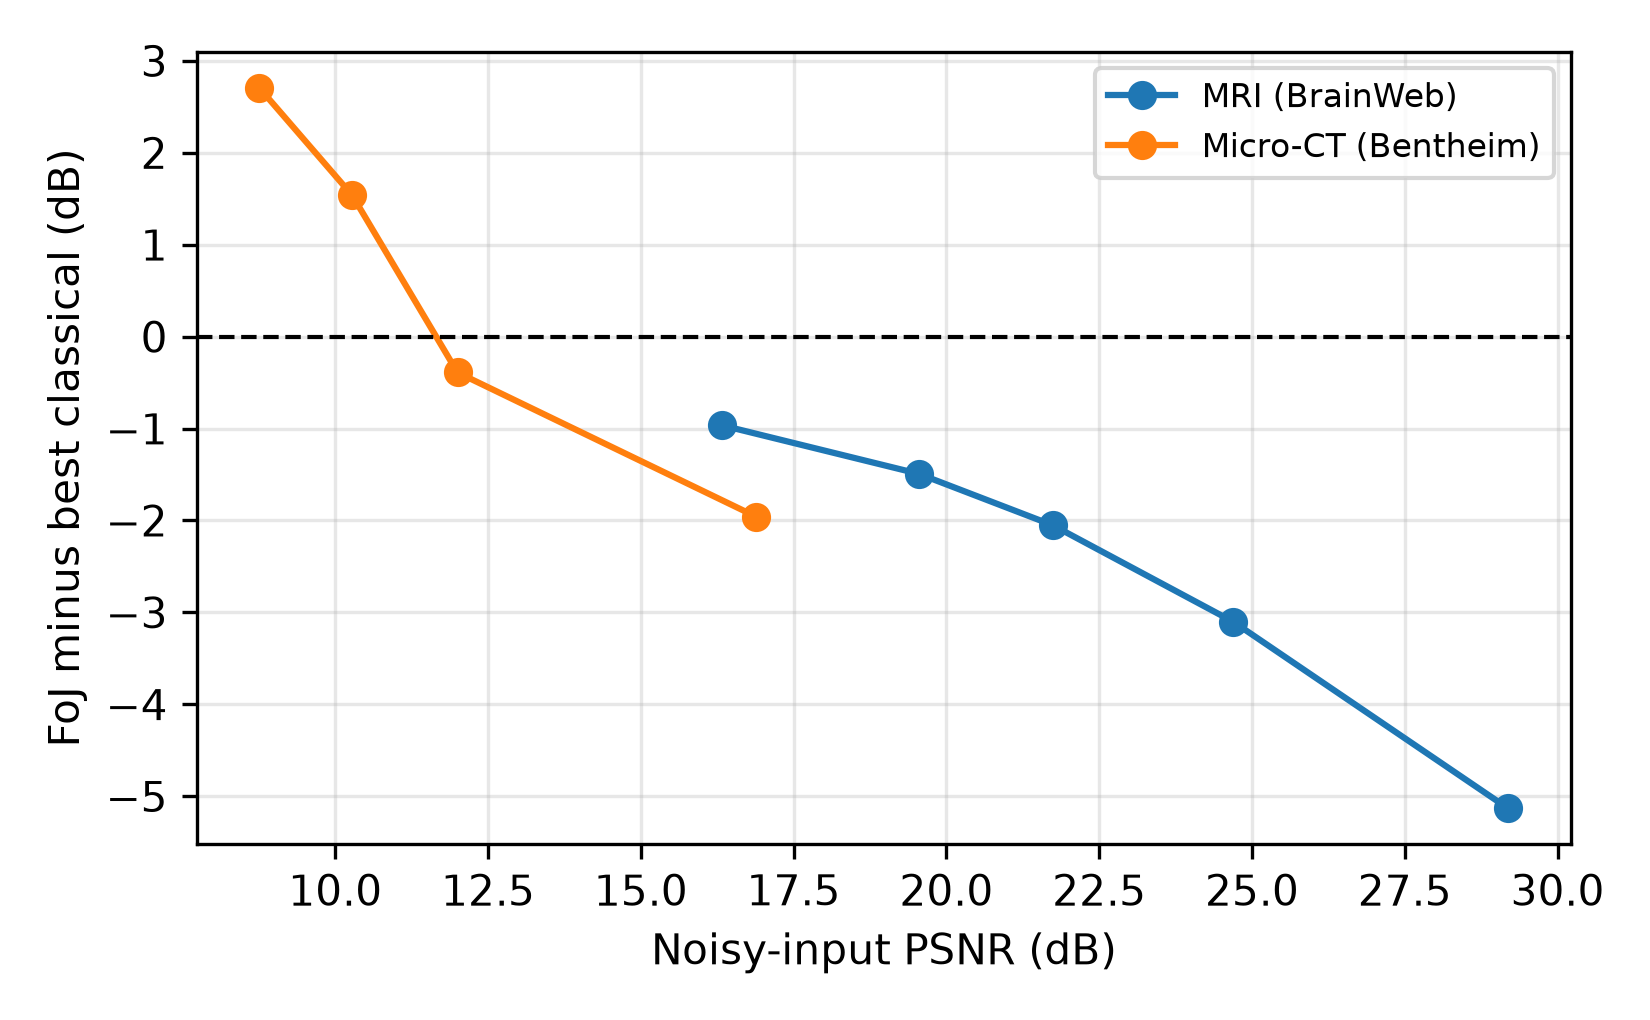
\includegraphics[width=0.72\linewidth]{fig_domains.png}
\caption{FoJ PSNR margin over the best classical denoiser versus input
PSNR. Above ${\approx}11$~dB input, classical filters are better; below
it, FoJ is better on piecewise-constant volumes.}
\label{fig:domains}
\end{figure}

%=====================================================================
\section{When does FoJ help?}

Each result above follows from the separable estimator of
Section~\ref{sec:mechanism} rather than standing alone
(Table~\ref{tab:factors}). The method succeeds when three conditions
hold together: the input is unbiased, the structure is piecewise-flat at
or above the patch scale, and the noise is high enough that the wedge
model's bias is paid for by the noise it removes. The micro-CT setting
is the one case in our study where all three hold.

\begin{table}[h]
\centering\small
\caption{The three requirements and the experiment that tested each.}
\label{tab:factors}
\begin{tabular}{>{\raggedright\arraybackslash}p{3.2cm}>{\raggedright\arraybackslash}p{5.7cm}>{\raggedright\arraybackslash}p{5.7cm}}
\toprule
Requirement & Evidence & Rule of thumb \\
\midrule
Unbiased input &
Clamping CGLS output to $[0,1]$ costs $2.7$--$4.3\dB$ and flattens the
patch-size trend. &
Feed FoJ an unclamped, bias-free input. \\[4pt]
Compatible structure &
Simplified projector flips the patch ordering at matched PSNR; smooth MRI
tissue trails a median filter by $1.0$--$5.1\dB$; sub-patch binary
features collapse FoJ to the mean ($7.1\dB$). &
Regions flat and larger than the patch; check both GT structure and
artifact structure. \\[4pt]
Low input SNR &
Micro-CT crossover at ${\approx}11\dB$ input; FoJ leads by $+1.5$ to
$+3.2\dB$ below it. &
Use FoJ where classical filters fail, not where they work. \\
\bottomrule
\end{tabular}
\end{table}

%=====================================================================
\section{Conclusion}

At its default configuration, 3D Field of Junctions reduces to an
independent per-patch wedge fit followed by overlap averaging. Its regime
of validity follows from that mechanism. The input must be unbiased:
clamping a reconstruction to $[0,1]$ costs up to $4.3\dB$ and nearly
eliminates the patch-size trend. The structure must be piecewise-flat at
or above the patch scale: smooth MRI tissue fails at every noise level,
and sub-patch-scale features collapse the output to the mean. The input
SNR must be low enough that the wedge model's approximation bias is paid
for by the noise it removes: on Bentheim sandstone micro-CT, FoJ
overtakes Gaussian, median, and TV denoisers below an input PSNR of about
$11\dB$ and leads by up to $3.2\dB$. The reported patch-size trend
reproduces under a faithful forward model but reverses under a different
projector, so hyperparameter conclusions for structural priors depend on
simulation fidelity. Outside the low-SNR, flat-structure regime, simple
classical filters are the better choice.

\paragraph{Future work.}
(1)~Dose sweeps (P50/P100/P1000) to test whether the optimal patch size
grows with noise level; (2)~additional objects to separate object scale
from noise; (3)~FoJ inside a proximal-gradient loop, as in the paper's
main CT experiment; (4)~BM4D and non-local-means baselines; (5)~real
scanner noise rather than synthetic corruption; (6)~junction-shaped
primitives inside the reconstruction rather than after it.

%=====================================================================
\begin{thebibliography}{99}

\bibitem{lepcha2025low}
D.~C.~Lepcha, B.~Goyal, A.~Dogra, K.~Vaghela, A.~Singh, K.~S.~R.~Kumar, and
D.~P.~Bavirisetti.
\newblock Low-dose computed tomography image denoising using pixel level
non-local self-similarity prior with non-local means for healthcare
informatics.
\newblock \emph{Scientific Reports}, 15(1):25095, 2025.

\bibitem{arnold2023low}
T.~C.~Arnold, C.~W.~Freeman, B.~Litt, and J.~M.~Stein.
\newblock Low-field {MRI}: clinical promise and challenges.
\newblock \emph{Journal of Magnetic Resonance Imaging}, 57(1):25--44, 2023.

\bibitem{turk2020promise}
M.~Turk and W.~Baumeister.
\newblock The promise and the challenges of cryo-electron tomography.
\newblock \emph{FEBS Letters}, 594(20):3243--3261, 2020.

\bibitem{rudin1992nonlinear}
L.~I.~Rudin, S.~Osher, and E.~Fatemi.
\newblock Nonlinear total variation based noise removal algorithms.
\newblock \emph{Physica D}, 60(1--4):259--268, 1992.

\bibitem{chambolle2004algorithm}
A.~Chambolle.
\newblock An algorithm for total variation minimization and applications.
\newblock \emph{Journal of Mathematical Imaging and Vision}, 20(1):89--97,
2004.

\bibitem{buades2005nonlocal}
A.~Buades, B.~Coll, and J.-M.~Morel.
\newblock A non-local algorithm for image denoising.
\newblock In \emph{CVPR}, 2005.

\bibitem{dabov2007image}
K.~Dabov, A.~Foi, V.~Katkovnik, and K.~Egiazarian.
\newblock Image denoising by sparse 3-D transform-domain collaborative
filtering.
\newblock \emph{IEEE Transactions on Image Processing}, 16(8):2080--2095,
2007.

\bibitem{zhang2017beyond}
K.~Zhang, W.~Zuo, Y.~Chen, D.~Meng, and L.~Zhang.
\newblock Beyond a Gaussian denoiser: Residual learning of deep CNN for
image denoising.
\newblock \emph{IEEE Transactions on Image Processing}, 26(7):3142--3155,
2017.

\bibitem{verbin2021foj}
D.~Verbin and T.~Zickler.
\newblock Field of Junctions: Extracting boundary structure at low SNR.
\newblock In \emph{ICCV}, 2021.

\bibitem{moeini2026foj3d}
N.~Moeini, N.~Kim, J.~Romberg, and S.~Fridovich-Keil.
\newblock 3D Field of Junctions: A noise-robust, training-free structural prior
for volumetric inverse problems.
\newblock In \emph{ECCV}, 2026. arXiv:2603.02149.
\newblock Code: \url{https://github.com/voilalab/3D-Field-of-Junctions}.

\bibitem{ulyanov2018deep}
D.~Ulyanov, A.~Vedaldi, and V.~Lempitsky.
\newblock Deep image prior.
\newblock In \emph{CVPR}, 2018.

\bibitem{zha2022naf}
R.~Zha, Y.~Zhang, and H.~Li.
\newblock {NAF}: Neural attenuation fields for sparse-view {CBCT}
reconstruction.
\newblock In \emph{MICCAI}, 2022.

\bibitem{noise2noise}
J.~Lehtinen, J.~Munkberg, J.~Hasselgren, S.~Laine, T.~Karras, M.~Aittala,
and T.~Aila.
\newblock Noise2Noise: Learning image restoration without clean data.
\newblock In \emph{ICML}, 2018.

\bibitem{filter2noise}
Y.~Sun, L.-S.~Schneider, M.~Gu, S.~Mei, C.~Ye, F.~Wagner, S.~Bayer, and
A.~Maier.
\newblock Filter2Noise: Interpretable self-supervised single-image
denoising for low-dose {CT} with attention-guided bilateral filtering.
\newblock arXiv:2504.13519, 2025.

\bibitem{polansky2024boundary}
M.~Polansky, C.~Herrmann, J.~Hur, D.~Sun, D.~Verbin, and T.~Zickler.
\newblock Boundary attention: Learning curves, corners, junctions and grouping.
\newblock In \emph{ECCV Workshops}, 2024.

\bibitem{zha2024r2gaussian}
R.~Zha, T.~J.~Lin, Y.~Cai, J.~Cao, Y.~Zhang, and H.~Li.
\newblock R$^2$-Gaussian: Rectifying radiative Gaussian splatting for
tomographic reconstruction.
\newblock In \emph{NeurIPS}, 2024.

\bibitem{biguri2016tigre}
A.~Biguri, M.~Dosanjh, S.~Hancock, and M.~Soleimani.
\newblock TIGRE: a MATLAB-GPU toolbox for CBCT image reconstruction.
\newblock \emph{Biomedical Physics \& Engineering Express}, 2(5):055010, 2016.

\bibitem{hestenes1952cg}
M.~R.~Hestenes and E.~Stiefel.
\newblock Methods of conjugate gradients for solving linear systems.
\newblock \emph{Journal of Research of the National Bureau of Standards},
49(6):409--436, 1952.

\bibitem{wang2003msssim}
Z.~Wang, E.~P.~Simoncelli, and A.~C.~Bovik.
\newblock Multiscale structural similarity for image quality assessment.
\newblock In \emph{Asilomar Conference on Signals, Systems and Computers}, 2003.

\bibitem{bentheim2015zenodo}
S.~Berg, H.~Ott, D.~Armstrong, A.~Schwing, J.~Humphrey, and R.~Necker.
\newblock High-resolution X-ray computed tomography images of Bentheim
sandstone (1~MPa, $5.854\,\mu\mathrm{m}$).
\newblock Zenodo, \url{https://doi.org/10.5281/zenodo.5548582}, 2021.

\bibitem{collins1998brainweb}
D.~L.~Collins, A.~P.~Zijdenbos, V.~Kollokian, J.~G.~Sled, N.~J.~Kabani,
C.~J.~Holmes, and A.~C.~Evans.
\newblock Design and construction of a realistic digital brain phantom.
\newblock \emph{IEEE Transactions on Medical Imaging}, 17(3):463--468, 1998.

\bibitem{neumann2020sandstones}
R.~Neumann, M.~Andreeta, and E.~Lucas-Oliveira.
\newblock 11 sandstones: raw, filtered and segmented data.
\newblock Digital Rocks Portal, \url{https://doi.org/10.17612/F4H1-W124}, 2020.

\end{thebibliography}

\end{document}
